		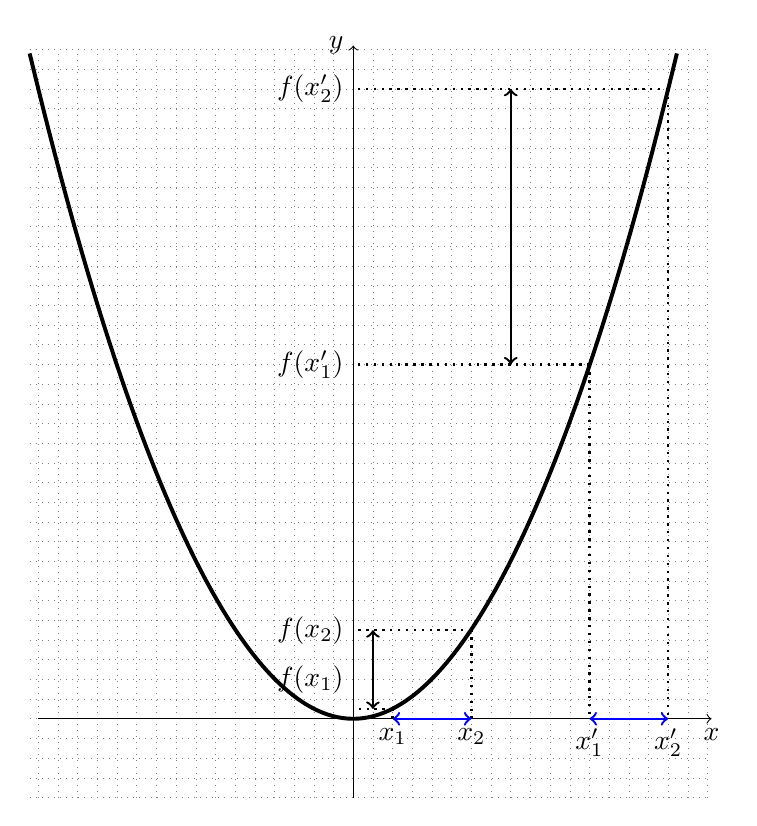
\begin{tikzpicture}
			% Рисуем сетку
			\draw[help lines, step=0.25, dotted]
			(-4.11,-1) grid (4.5,8.5);
			% Начало координат
			\draw[->, thin] (-4,0) -- (4.55,0)
			node[below] {$x$}; % Ox
			\draw[->, thin] (0,-1) -- (0, 8.55)
			node[left] {$y$}; % Oy
			
			\draw[line width =.05cm](-4.11, 8.45) parabola bend (0, 0)(4.11, 8.45);
			
			\draw[dotted, line width =.03cm] (0.5, 0) -- (0.5, 0.125);
			\draw[dotted, line width =.03cm] (0.5, 0.125) -- (0, 0.125);
			\draw[dotted, line width =.03cm] (1.5, 0) -- (1.5, 1.125);
			\draw[dotted, line width =.03cm] (1.5, 1.125) -- (0, 1.125);
			\draw[dotted, line width =.03cm] (3, 4.5) -- (3, 0);
			\draw[dotted, line width =.03cm] (3, 4.5) -- (0, 4.5);
			\draw[dotted, line width =.03cm] (4, 8) -- (0, 8);
			\draw[dotted, line width =.03cm] (4, 8) -- (4, 0);

            \draw[<->, line width =.03cm] (0.25, 0.125) -- (0.25, 1.125);
            \draw[<->, line width =.03cm] (2, 4.5) -- (2, 8);

            \draw[<->, line width =.03cm, blue] (0.5, 0) -- (1.5, 0);
            \draw[<->, line width =.03cm, blue] (3, 0) -- (4, 0);
            
			
			\node[below] at (0.5, 0) {$x_{1}$};
            \node[below] at (1.5, 0) {$x_{2}$};
			\node[below] at (3, 0) {$x_{1}'$};
            \node[below] at (4, 0) {$x_{2}'$};
			\node[left] at (0, 1.125) {$f(x_{2})$};
			\node[left] at (0, 0.5) {$f(x_{1})$};
   		\node[left] at (0, 4.5) {$f(x_{1}')$};
			\node[left] at (0, 8) {$f(x_{2}')$};

		\end{tikzpicture}